\documentclass[conference]{IEEEtran}
\IEEEoverridecommandlockouts
% The preceding line is only needed to identify funding in the first footnote. If that is unneeded, please comment it out.
\usepackage{cite}
\usepackage{amsmath,amssymb,amsfonts}
\usepackage{algorithmic}
\usepackage{graphicx}
\usepackage{textcomp}
\def\BibTeX{{\rm B\kern-.05em{\sc i\kern-.025em b}\kern-.08em
    T\kern-.1667em\lower.7ex\hbox{E}\kern-.125emX}}
\begin{document}

\title{CENG435 Group 60 TP Part-1 Report\\
%{\footnotesize \textsuperscript{*}Note: Sub-titles are not captured in Xplore and
%should not be used}
\thanks{}
}

\author{\IEEEauthorblockN{\textsuperscript{} Kadir Burak Tokmak}
\IEEEauthorblockA{\textit{} 
\textit{ID :2036200} \\
}
\and
\IEEEauthorblockN{\textsuperscript{} Emrah Kosen}
\IEEEauthorblockA{\textit{}
\textit{ID:1942317}\\
}

}

\maketitle





\section{Introduction}
\large

For this project we are working with a topology consisting of 5 nodes with 8 links. Each link has its own interface and subnet with each containing 2 hosts. \\
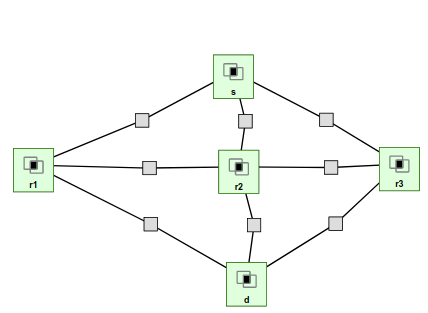
\includegraphics[width = 90mm, height = 80mm]{topology.png}\\ \qquad \\


In this topology links are can be defined as:\\

$\bullet$R1-R2 link: 10.10.8.0/24 Subnet with 100kbs bandwidth\\

$\bullet$R2-R3 link 10.10.6.0/24 Subnet with 100kbs bandwidth\\

$\bullet$R1-D link 10.10.4.0/24 Subnet with 1000kbs bandwidth\\

$\bullet$R2-D link 10.10.5.0/24 Subnet with 1000kbs bandwidth\\

$\bullet$R3-D link 10.10.7.0/24 Subnet with 2000kbs bandwidth\\

$\bullet$R1-S link 10.10.1.0/24 Subnet with 1000kbs bandwidth\\

$\bullet$R2-S link 10.10.2.0/24 Subnet with 1000kbs bandwidth\\

$\bullet$R3-S link 10.10.3.0/24 Subnet with 2000kbs bandwidth\\

Topology is contained in virtual machines and access to these virtual machines are done via ssh connections.\\

At start random delays are added to interfaces of R1-R2 nodes with given configure files.\\

Two major scripts needs to be implemented in this project. First script will be discovery script and will find round-trip times between links and find shortest path between S-D nodes. Second script will be experiment script and will be using the shortest path found in discovery scripts to implement its routing between S-D nodes. After routing is implemented experiment scripts will calculate end to end delays with 20ms+-5ms, 40ms+-5ms, 50ms+-5ms separately.\\ \quad \\

\section{Design}

In the topology there are 8 links. Each link's round-trip time needs to be calculated from one of the nodes. Two roles defined for nodes corresponding each link. \\

Sender Role: These nodes will take the time data that has been sent to them and send the data back to the sender. They do not calculate the time delay.\\

Reciever Role: These nodes will send their current time to sender nodes and will recieve back the time data from sender nodes. They will calculate the time difference and find round-trip times. Found round-trip times will be send to D node after messaging period ends.\\

In this design S node will be sender for S-R1 link, S-R2 link and S-R3 link \\

$\bullet$R1 node will be reciever for S-R1 link, sender for R1-D link and sender for R1-R2 link.\\

$\bullet$R2 node will be reciever for S-R2 link, reciever for R1-R2 link, sender for R2-R3 link and sender for R2-D link.\\

$\bullet$R3 node will be reciever for R2-R3 link, reciever for R3-S link and sender for R3-D link.\\

$\bullet$D node will be reciever for R1-D link, reciever for R2-D link and reciever for R3-D link.\\

After messaging periods are done found round-trip times for links will be sent to D by R1-R2-R3. D node then will make a linkcosts.txt to store all link costs. D node will also calculate shortest path between S-D with Dijkstra Algorithm. Calculated shortest path will be send to each node and will be saved to routelist.txt in each node. This route list will be used in experimental scripts to decide routing path. Experimental scripts will need this routelist to be functional. In experimental scripts nodes in the shortest path will forward the time data between S-D back forth.\\ \quad \\

\section{Implementation}


For implementing the design python language is used. Socket, thread and time libraries are also imported for our later use.\\

In Socket library UDP sockets are defined then bind to an address and a port for use. Different ports are used for sending and reciving in this implementation. Socket fuction sendto used for sending udp packets and oscket fuction recvfrom with a buffer used for reciving udp packets.\\

Nodes are given an index number for ease of use later on in routing and script works. S,R1,R2,R3,D nodes are given index number 0,1,2,3,4 \\

For every script matrix of IP addresses are used to refer to connections between nodes. Example: Matrix [1][4] can be used for the connection from R1 to D\\

First to fill the sender and reciever roles of the Sender and Reciever functions were defined to use in discovery scripts of the nodes. \\


Sender function: This fuctions recieves the amount of messages need to be sent and required addresses and the port as argument. Sender fuctions sends a "ready" message first to activate reciever function in the target node. Following "ready" message sender sends the amount of message that will follow up and reciever function will itarate on this amount. Sender then recieves the time from reciever node and sends it back to reciever node. Sender nodes functions are over at this point. For any possibility of packet loss timeout is implemented for socket to close itself. \\

Reciever fuction: This function recieves the corresponding addresses and ports as an argument. Reciever function waits to recieve "ready" message from sender node then it recieves the amount of messages that will be sent. 100 messages are used in this implementation with the capability of increasing to any number. Reciever functions sends its current time and recieves it back. After that it calculates the time difference between recieved and current time to find the round-trip time of the corresponding link. For R1-R2-R3 nodes found link costs are send to D node for later calculation in that node. For any possibility of packet loss timeout is also implemented for socket to close itself.\\

Nodes in this project needs to send and recieve messages at the same time. Since an operation like waiting for UDP packet stalls our program, threading is implemented in the implementation of the scripts. Defined functions are called with threading and joined after messaging period ends. For every send or recieve purpose nodes open a thread for that need. These steps allowed the scripts to send and recieve the messages at the same time. Running scripts starts their threads immediately and will look for their corresponding node.\\

Links costs needs to be collected at one location before shortest path is calculated. In this implementation D node is selected for this purpose. D recieves the costs of links R1-S, R2-S, R3-S, R1-R2, R2-R3 before its messaging period ends.\\

Found round-trip times after 100 message sequence can be seen in table below.\\ \qquad \\

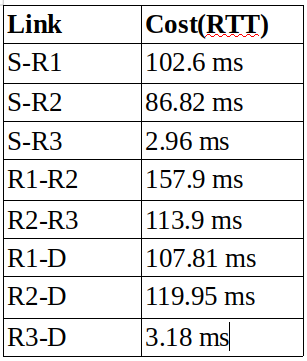
\includegraphics[width = 80mm, height = 95mm]{rtt.png}\\ \qquad \\

Finding shortest path is important for our discoery scripts. To find the shortest path between S-D Dijkstra’s shortest path algorithm is implemented with the link cost data. This algorithm is implemented at D node.\\

The Dijkstra algorithm chooses the shortest path first that is connected to S. These paths can be implemented as vertices. Algorithm then checks for other vertices to find if reaching to next point is smaller than already existing min distance. Min distance start with "max" value so first path will be registered for shortest first then can be changed later. If a path is smaller than than previous path that node's parent set with the corresponding path. Parents list show node's next hop address while reaching from S to D.(For more detailed work of the algorithm comments in "d.py" in discoveryscripts can be examined)\\

After running the script we can see the first parent list as [-1, 0, 0, 0, 3] . If we go through by index number we gave at the start we can see that parent of D is 3 which is R3. If we look at parent[3] result is 0 which means parent of R3 is S. With these specifications a routelist is made an send to all other nodes. For this situation [-1, -2, -2, 0, 3] is send as a route list for all nodes. Nodes look up to their index number in this list to decide if they are in the shortest path or not. -2 value means that  node is not in the shortest path and won't include itself in the experiment part. If nodes is in the shortest path it will act accordingly during the experimental phase. After sending this route list to all nodes, every nodes makes a routelist.txt that will be used later on with the experiment part of the project.\\

For experimental all scripts will be the same with the exception of hostID numbers. Script will work according to routelist.txt and hostID. If a host finds itself in the route in the routelist.txt it will open ports accordingly to listen and send packets from the parent node to destination node. If node find itself to be not in the route script will terminate. In this experiment R1-R2 will terminate after they look into the routelist while R3 will open ports to both listen and send traffic between S-D. S sends its current time as data to R3 and this data will be forwarded to D which D will recieve and forward back to R3-S. S at this point will calculate the time difference and will find round-trip time values. For end to end delay we will need half of this number. Experimental script prints every delay in a new line for the use of making a graph.\\

Before making the experiments network emulations delays needed to be implemented. For the experiments in R3 node delays are implemented in two network interfaces. One with between S node other with between D node.\\

Configuration used for network delay can be seen in the picture below.\\\qquad \\

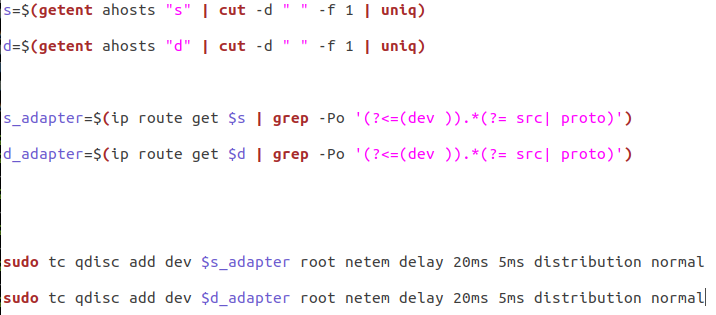
\includegraphics[width = 80mm, height = 35mm]{configure.png}\\ \qquad \\

Before any delay is implemented we find with experimental scripts that end-to-end delay between is 95\% Confidence Interval: 0.96 ± 0.0784 ms\\

Since this implementation of network delay is first we use "add" function for the 20ms+-5ms delay. Normal distribution is used for the delay. For the 40ms+-5ms and 50ms+-5ms delay "change" functions of the network emulation delay will be used since we will change the existing delays.\\


After first delay is implemented for experiment 1. Experiment scripts are run. At the end of experiments with 50 messages sent and recieved back by S end-to-end delay can be calculated as 95\% Confidence Interval: 21.3 ± 0.809 ms.\\ 

Network emulation delay is changed to 40ms+-5ms for our second experiment. After the experiment scripts running we find a end-to-end delay as 95\% Confidence Interval: 40.8 ± 0.843 ms .\\

For the third experiment r3 delays are changed to 50ms+-5ms with netem commands. 50 messages sent and recieved again with the calculation of end-to-end delay found as 95\% Confidence Interval: 52 ± 0.965.\\

End-to-end delay's relation with network emulation is seen in graph below.


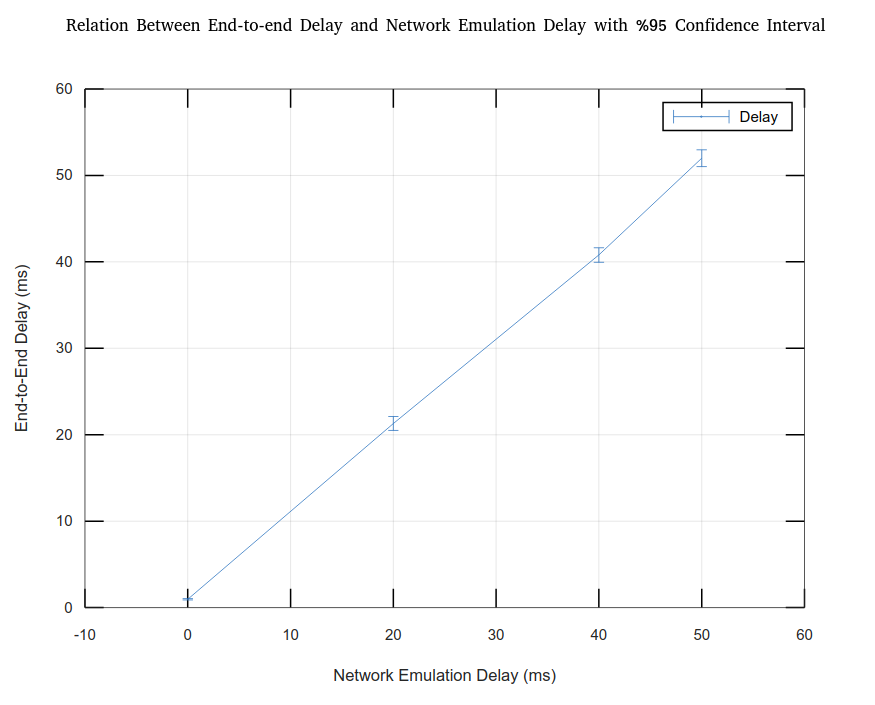
\includegraphics[width = 100mm, height = 70mm]{end_delay.png}\\ \qquad \\

Since the starting delay was around 1ms for both S-R3 and D-R3 links. Implementing any delay to those interfaces will make new delay addition to the first delay. We can see that avarages of end-to-end delays are very close to "nertwork emulation delay + 1ms" formula. \\

Added delay on R3 interfaces only in effect when R3 is sending packets. So while packets are traveling S to R3 and R3 to D they only get effected by this delay once when leaving R3 to D. Same delay can be experienced when packets are traveling D to R3 and R3 to S. Packets will be delayed again while leaving R3 to S.\\ 

\section{Conclusion}

Project has been concluded with our experiments done and results implemented in end-to-end delay with relation to delay emulation graph. Implementing socket applications, finding link costs, implementing shortest path algorith with link costs and application level routings were points of our implementation. For experiments phase usage and understanding of network emulations delays were important. With the results we recieved Part-1 of the Term Project is concluded. Please take a look at the files inclueded. For running the scripts inclueded check ReadMe.txt.

\end{document}
